\documentclass[twoside]{article}
\setlength{\oddsidemargin}{0.25 in}
\setlength{\evensidemargin}{-0.25 in}
\setlength{\topmargin}{-0.6 in}
\setlength{\textwidth}{6.5 in}
\setlength{\textheight}{8.5 in}
\setlength{\headsep}{0.75 in}
\setlength{\parindent}{0 in}
\setlength{\parskip}{0.1 in}

\usepackage{graphicx}
\usepackage{url}

%
% The following commands sets up the lecnum (lecture number)
% counter and make various numbering schemes work relative
% to the lecture number.
%
\newcounter{lecnum}
\renewcommand{\thepage}{\thelecnum-\arabic{page}}
\renewcommand{\thesection}{\thelecnum.\arabic{section}}
\renewcommand{\theequation}{\thelecnum.\arabic{equation}}
\renewcommand{\thefigure}{\thelecnum.\arabic{figure}}
\renewcommand{\thetable}{\thelecnum.\arabic{table}}
\newcommand{\dnl}{\mbox{}\par}

%
% The following macro is used to generate the header.
%
\newcommand{\lecture}[4]{
  \pagestyle{myheadings}
  \thispagestyle{plain}
  \newpage
  \setcounter{lecnum}{#1}
  \setcounter{page}{1}
  \noindent
  \begin{center}
  \framebox{
     \vbox{\vspace{2mm}
   \hbox to 6.28in { {\bf CMPSCI~630~~~Systems
                       \hfill Fall 2019} }
      \vspace{4mm}
      \hbox to 6.28in { {\Large \hfill Lecture #1  \hfill} }
%       \hbox to 6.28in { {\Large \hfill Lecture #1: #2  \hfill} }
      \vspace{2mm}
      \hbox to 6.28in { {\it Lecturer: #3 \hfill Scribe: #4} }
     \vspace{2mm}}
  }
  \end{center}
  \markboth{Lecture #1: #2}{Lecture #1: #2}
  \vspace*{4mm}
}

%
% Convention for citations is authors' initials followed by the year.
% For example, to cite a paper by Leighton and Maggs you would type
% \cite{LM89}, and to cite a paper by Strassen you would type \cite{S69}.
% (To avoid bibliography problems, for now we redefine the \cite command.)
%
\renewcommand{\cite}[1]{[#1]}

% \input{epsf}

%Use this command for a figure; it puts a figure in wherever you want it.
%usage: \fig{NUMBER}{FIGURE-SIZE}{CAPTION}{FILENAME}
\newcommand{\fig}[4]{
           \vspace{0.2 in}
           \setlength{\epsfxsize}{#2}
           \centerline{\epsfbox{#4}}
           \begin{center}
           Figure \thelecnum.#1:~#3
           \end{center}
   }

% Use these for theorems, lemmas, proofs, etc.
\newtheorem{theorem}{Theorem}[lecnum]
\newtheorem{lemma}[theorem]{Lemma}
\newtheorem{proposition}[theorem]{Proposition}
\newtheorem{claim}[theorem]{Claim}
\newtheorem{corollary}[theorem]{Corollary}
\newtheorem{definition}[theorem]{Definition}
\newenvironment{proof}{{\bf Proof:}}{\hfill\rule{2mm}{2mm}}

% Some useful equation alignment commands, borrowed from TeX
\makeatletter
\def\eqalign#1{\,\vcenter{\openup\jot\m@th
 \ialign{\strut\hfil$\displaystyle{##}$&$\displaystyle{{}##}$\hfil
     \crcr#1\crcr}}\,}
\def\eqalignno#1{\displ@y \tabskip\@centering
 \halign to\displaywidth{\hfil$\displaystyle{##}$\tabskip\z@skip
   &$\displaystyle{{}##}$\hfil\tabskip\@centering
   &\llap{$##$}\tabskip\z@skip\crcr
   #1\crcr}}
\def\leqalignno#1{\displ@y \tabskip\@centering
 \halign to\displaywidth{\hfil$\displaystyle{##}$\tabskip\z@skip
   &$\displaystyle{{}##}$\hfil\tabskip\@centering
   &\kern-\displaywidth\rlap{$##$}\tabskip\displaywidth\crcr
   #1\crcr}}
\makeatother

% **** IF YOU WANT TO DEFINE ADDITIONAL MACROS FOR YOURSELF, PUT THEM HERE:



% Some general latex examples and examples making use of the
% macros follow.

\begin{document}

%FILL IN THE RIGHT INFO.
%\lecture{**LECTURE-NUMBER**}{**DATE**}{**LECTURER**}{**SCRIBE**}
\lecture{3}{September 10}{Emery Berger}{Arta Razavi}

\section{Memory Hierarchy}

\begin{figure}[h!]
  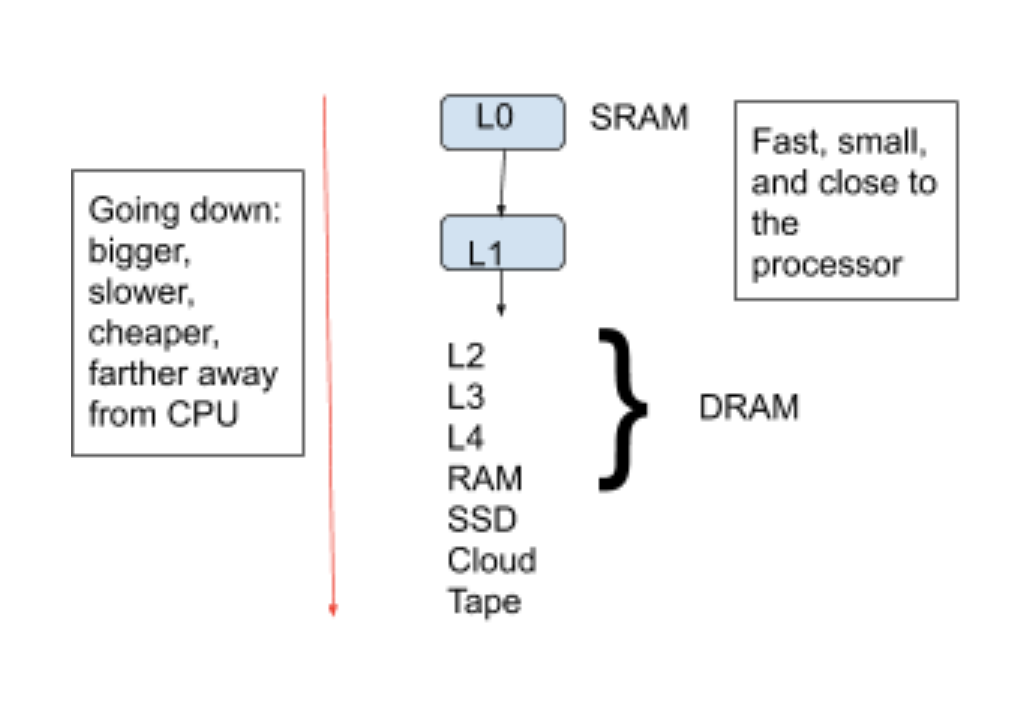
\includegraphics[width=\linewidth]{fig1.png}
  \caption{memory hierarchy}
  \label{fig:fig1}
\end{figure}

\textbf{Non volatile Memory (NVM):} persistent, when power is turned off the memory is still there. This is viewed as a new possible replacement for RAM
\newline
\textbf{transparency:} programs running on a computer do not know how many levels of cache there are or how big they are or anything about memory. There is an abstraction where programs think they are running on RAM.  
\newline\newline
C and C++ have direct access to virtual addresses but programming languages like Python, Java, and JavaScript do not.
\newline

\section{Cache Lines}
\begin{figure}[h!]
  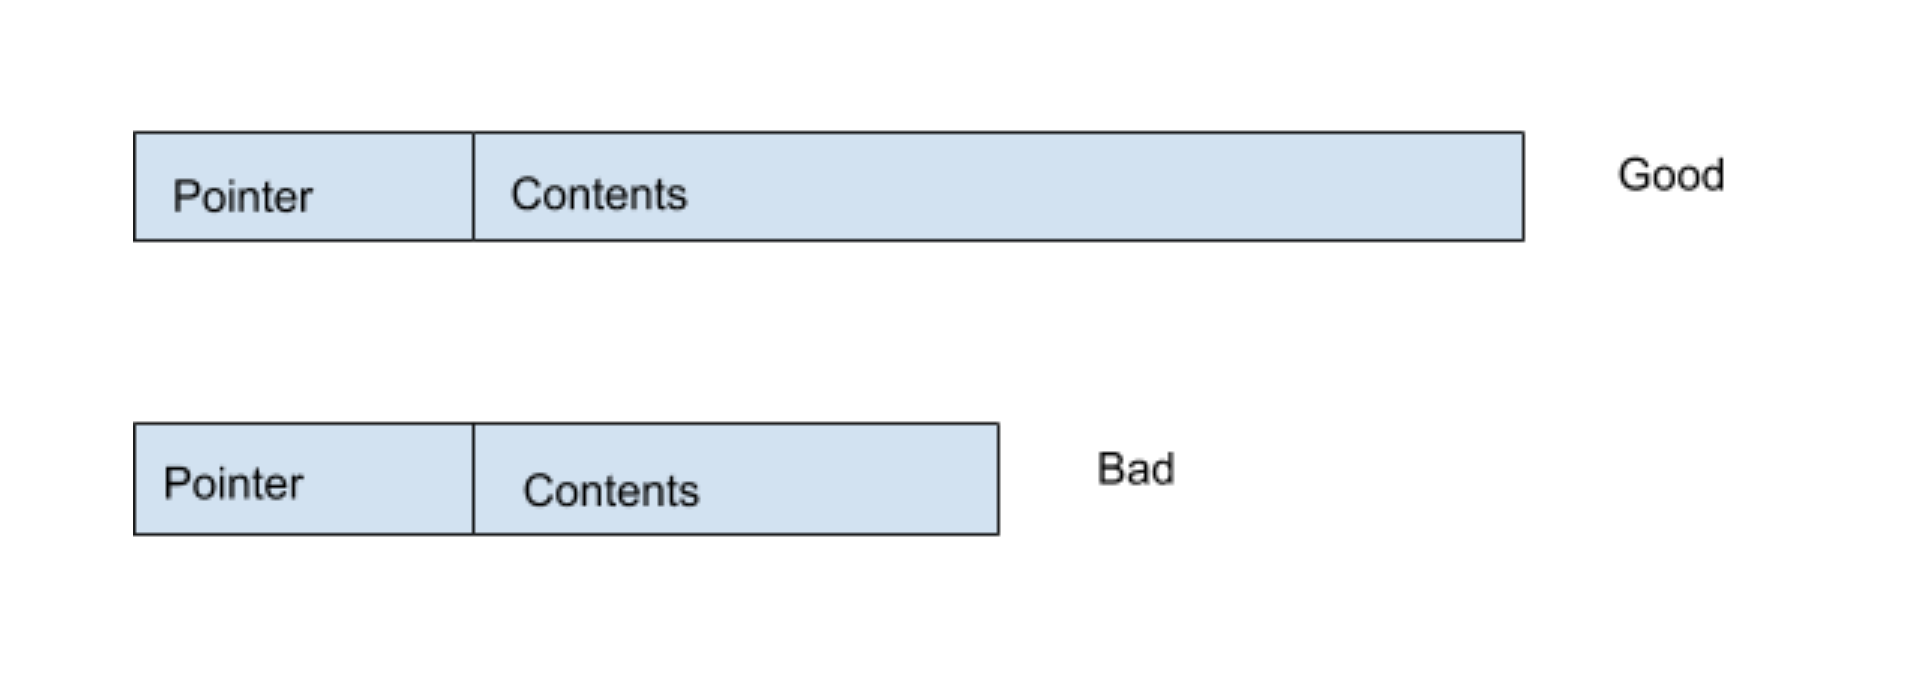
\includegraphics[width=\linewidth]{fig2.png}
  \caption{cache lines}
  \label{fig:fig2}
\end{figure}
There is a directory for which things are present in the cache. In the directory addresses are stores as pointers which point to a bunch of memory (contents). These contents are known as cache lines. Cache Lines are usually large, this amortizes management overhead of storing pointer addresses known as metadata. We want the overhead of storing pointer addresses to be smaller so we take larger chunks of content as cache lines. We wish for the size of the data to be larger than the size of the metadata. 
\newline
Addresses are rounded up to multiples 128 or 256 bits and you store that chunk. If asking for address 3 its going to be rounded to cache line 0 and 259 would return cache line 256. 
\section{Modern Chip}
\begin{figure}[h!]
  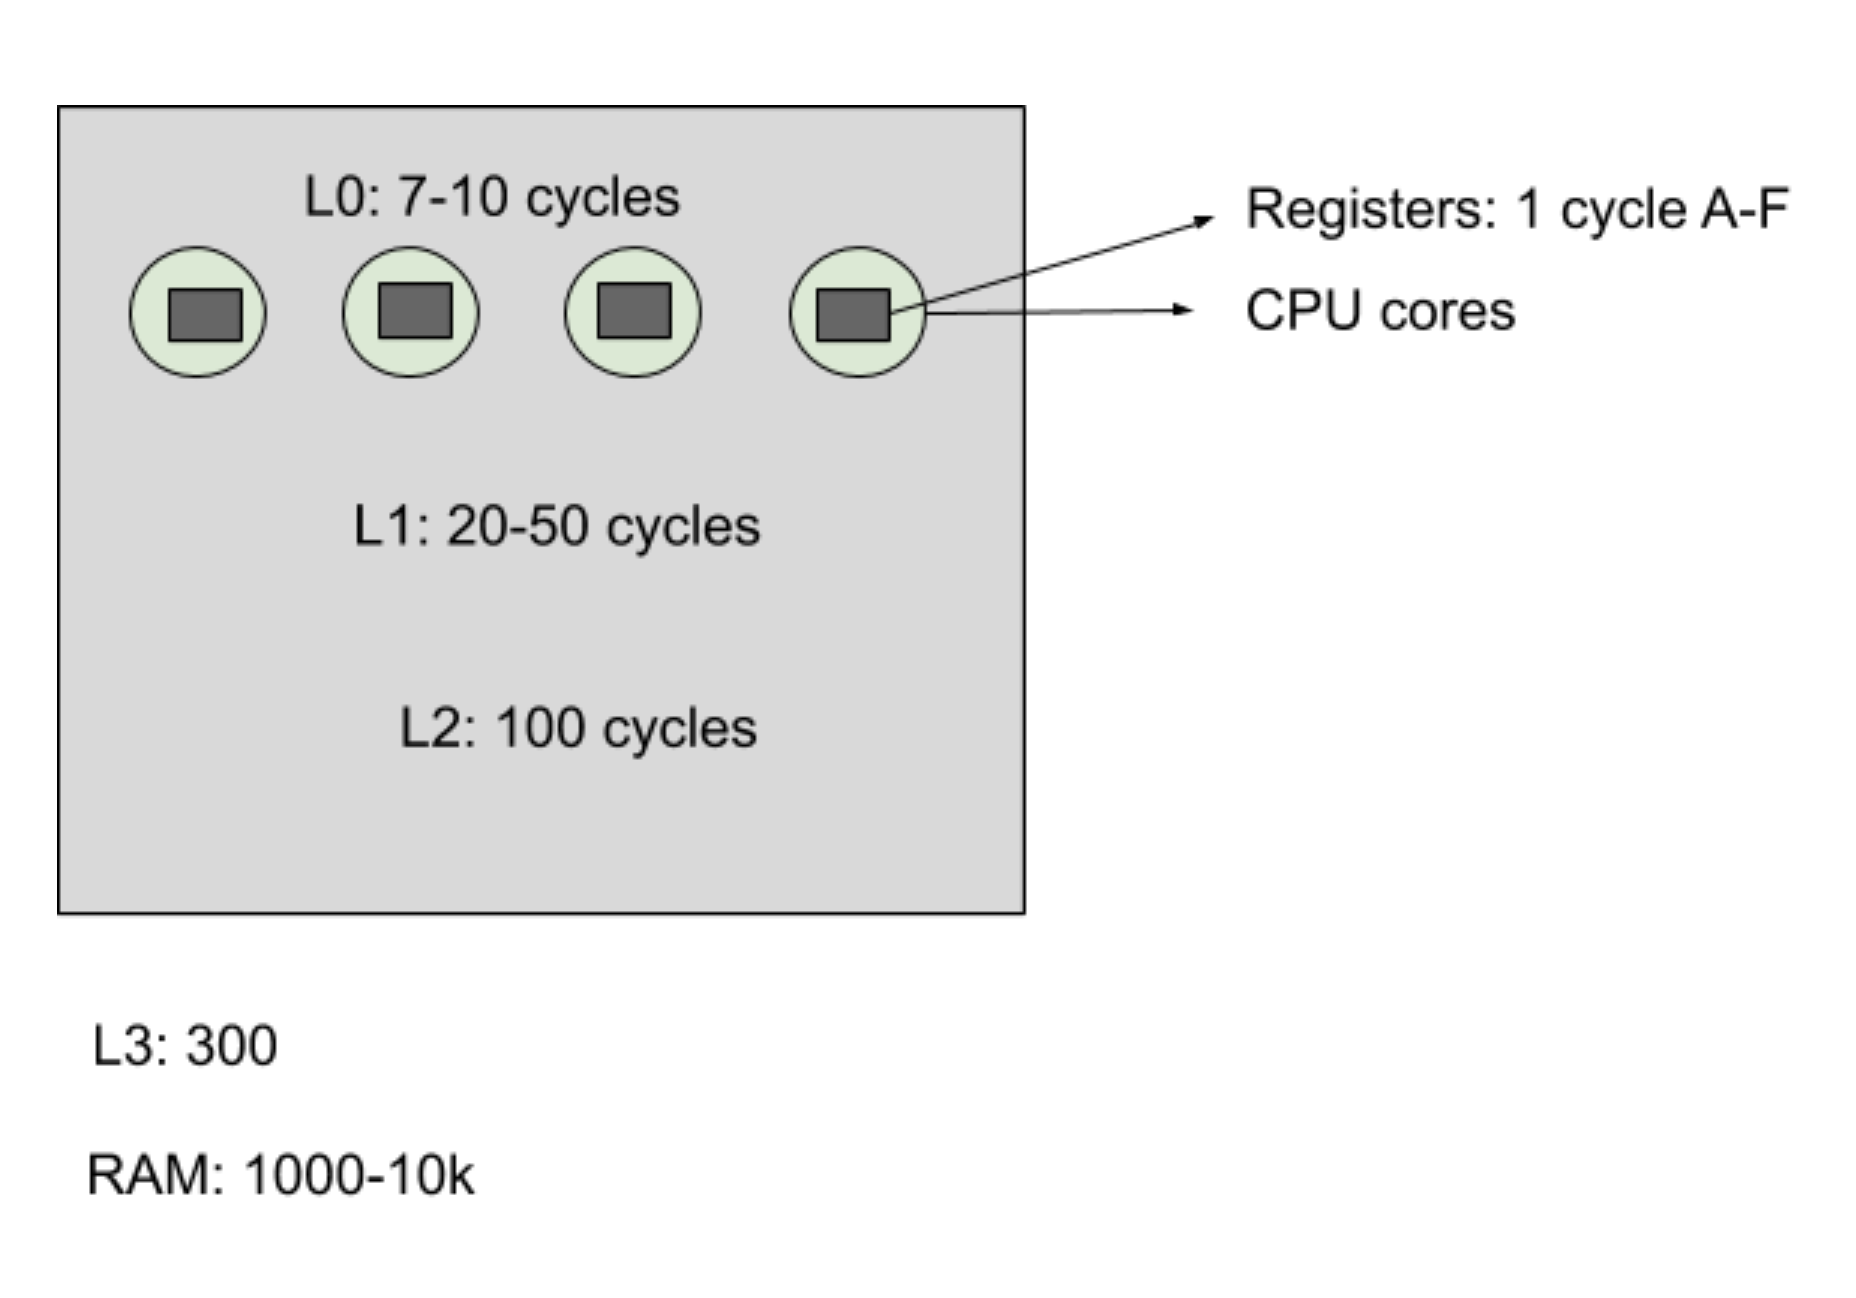
\includegraphics[width=\linewidth]{fig3.png}
  \caption{modern chip}
  \label{fig:fig3}
\end{figure}

CPU cores on modern chips each have their own individual caches as well as shared caches between pairs.
\newline
\textbf{Die Stacking:} The idea if that instead of having chips be on the same level stack them on top of each other to promote closeness. Less communication and more proximity of data to the chip. 
\newline
\textbf{Bus:} The way you get contents on the chip from the RAM and back. CPUs are spinning fast and there are many cores and they are all working hard but everything is bottle necked by the bus.  
\newline
\textbf{Registers:} Inside CPU there are registers which are faster memory that is accessible in one cycle (this is even faster than L0). They are assigned named variables A-F and you can read from and write to them. 
\newline

\section{Cache Storage}
\begin{figure}[h!]
  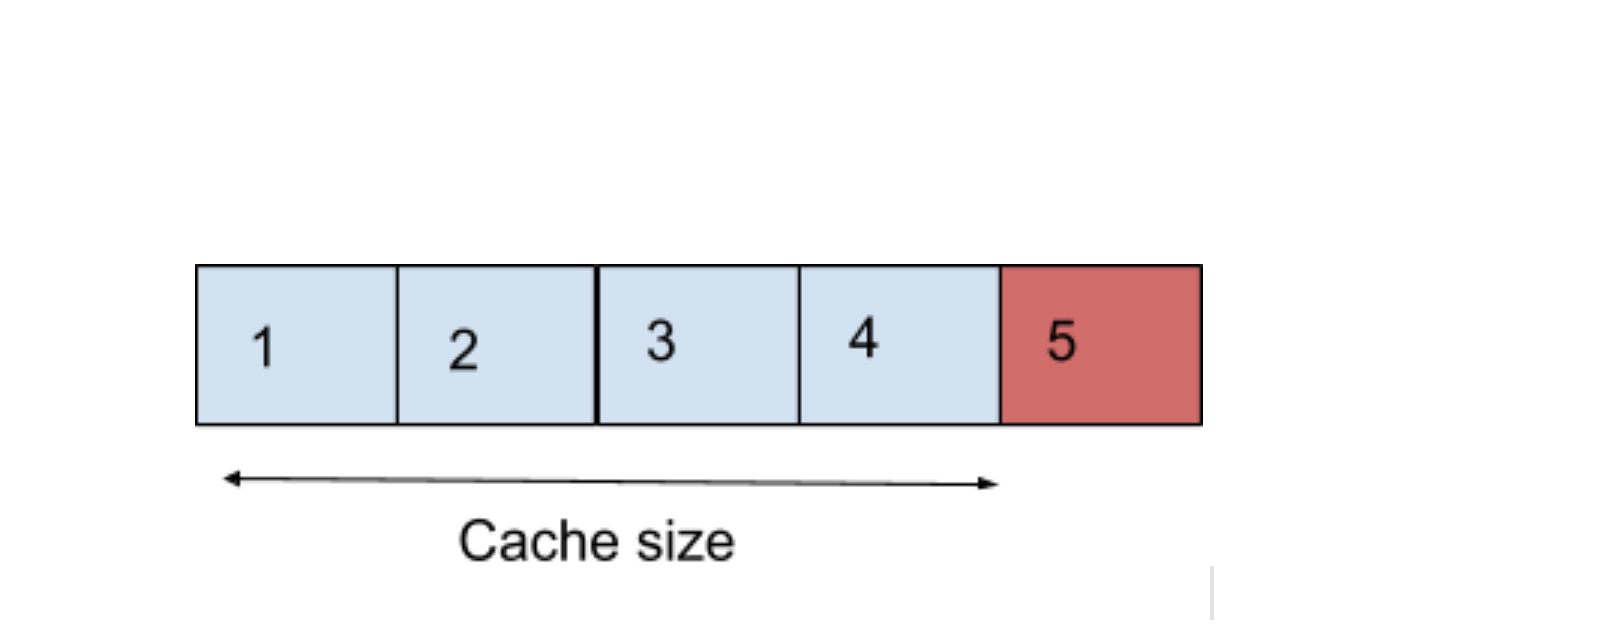
\includegraphics[width=\linewidth]{fig4.png}
  \caption{cache storage}
  \label{fig:fig4}
\end{figure}
CPU asks for a byte from an address then at first it asks L0 and if L0 doesn't have it then L1 and so on and if none of them have it eventually the CPU asks the RAM. Where is this content going to go after it was retrieved from RAM?
\newline
\textbf{Inclusive:} every cache level has a super set of data addresses stored in (level - 1). 
\newline
\textbf{LRU:} caches get filled up pretty quickly so we must use a replacement policy to move new data in and old data out of caches. The standard policy is least recently used (but not really there is a variation of this). As caches grow a bigger and bigger LRU is not favored because we do not want to be doing a linear search to find least recently used items.
\newline
\textbf{Exclusive:} Data is only stored in one level of cache. If data is evicted and we need access to it again we might have to go all the way back to RAM to get that data again (bad). 
\newline
\textbf{Latency:} The time spent waiting for data. Caches are a way to hide latency. 
\newline\newline
As seen in Figure 3.4: Say we have 5 chunks of data but only 4 spots in our cache. If we access the data in order 1,2,3,4,5 when 5 comes in 1 is evicted. If we circle back and ask for the data again from the beginning we would have to get every piece again from RAM because based on the LRU policy each one would get evicted right before its needed again. This is the worst case scenario for the exclusive policy. The inclusive policy performs better in this situation because there are multiple copies of the data stored across multiple caches.

\section{Multiple Processors/Cores}
\begin{figure}[h!]
  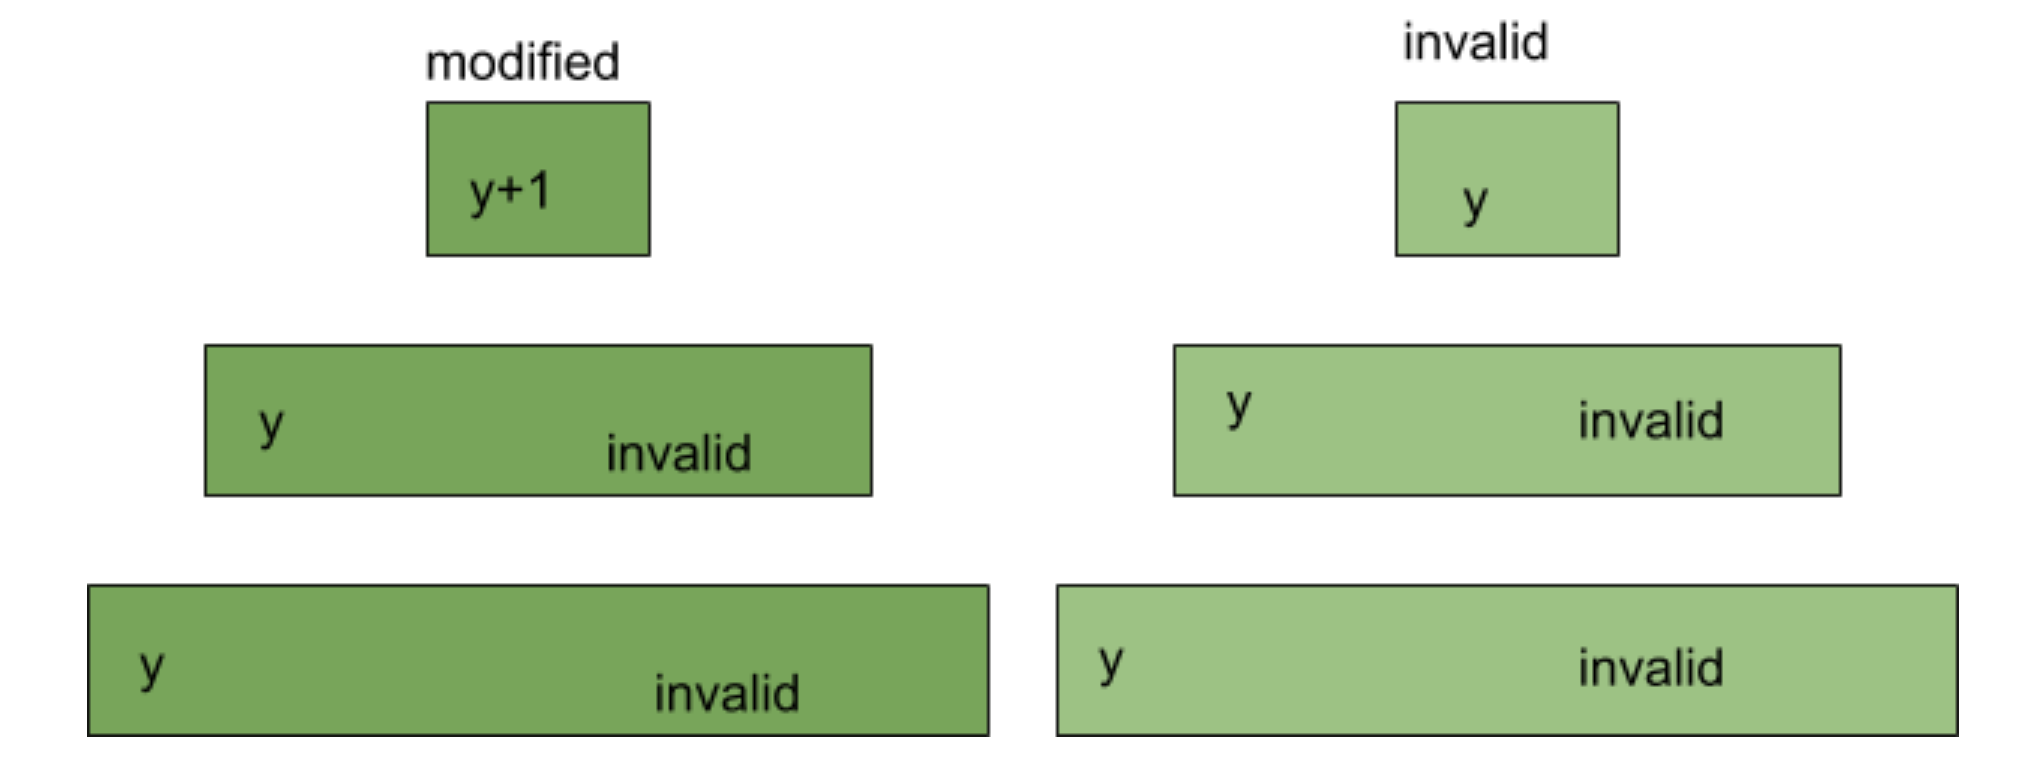
\includegraphics[width=\linewidth]{fig5.png}
  \caption{multiple processors}
  \label{fig:fig5}
\end{figure}
Suppose there are two processors and they are both storing values for the variable y. When y gets modified in one processor then the other values of y stored in the other caches becomes invalid.
\newline
\textbf{Coherence:} Everyone in the world must see the same view. The processor assures everything has the same view of memory in the machine at all times.
\newline\newline
There are different policies for when data gets propagated down levels of cache
\newline
\textbf{Write back:} changes only local (faster & most typically used)
\newline
\textbf{Write through:} changes are propagated all the way down the hierarchy (slower)

\section{MESI Protocol} 
A write back protocol that to keeps track of modified data and sync up memory.  This is because if there has been a modification made to data it eventually needs to make its way out to RAM. This has 2 bits that determine the value these bits signify 4 variables:
\newline
\textbf{Modified (M):} The data is only present in the current cache and it has been modified (M) from value that was stored in memory. This change needs to be propagated to main memory before allowing any farther read of the no longer valid memory. If a write back occurs this changes to shared state (S).
\newline
\textbf{Exclusive (E):} The data is only present in the current cache but it matches the data in main memory. This can respond to read calls.
\newline
\textbf{Shared (S):} This data may be present in other caches on the machine. The data matches main memory.
\newline
\textbf{Invalid (I):} This data is invalid and does not match main meory.
\newline
If the 2 bits are modified and exclusive it means I changed the data and I'm the only one that has a copy of it.
\newline
If the 2 bits are shared and invalid it means Several CPUs have an unmodified version of it. (Trash)
\newline
In an inclusive cache every single level is implicated but in an exclusive cache only one level is implicated. When this type of sharing across multiple processors is taking place an exclusive cache performs much faster.

\section{Approximate LRU Implementation}
\begin{figure}[h!]
  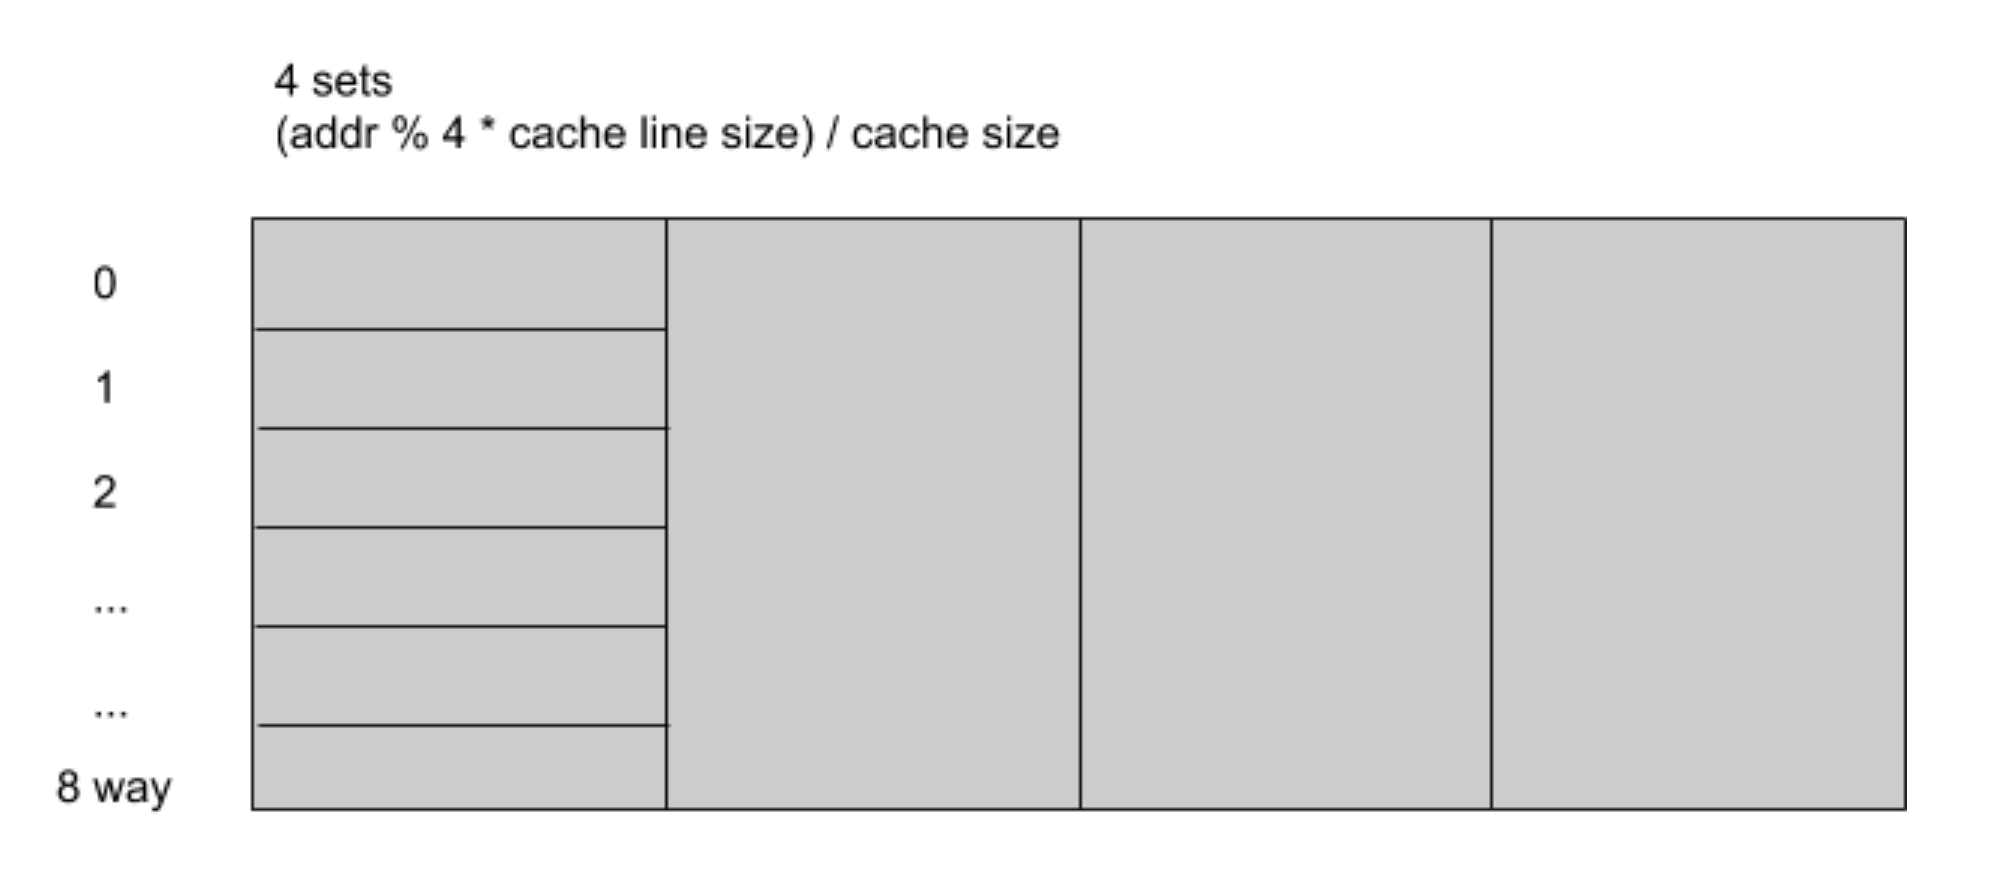
\includegraphics[width=\linewidth]{fig6.png}
  \caption{approximate LRU}
  \label{fig:fig6}
\end{figure}
Storing a bunch of addresses and doing a linear search of all addresses upon eviction is not efficient. Instead, we divide up addresses by hashing them into different bins which are refereed to as sets. Now memory address management is divided up into groups and there is only a fixed number of addresses in each set to track instead of linearly scanning all addresses. In Figure3.6 above in a 8 way set we are only performing LRU on 8 addresses instead of all of them.
\newline
We do this by storing counters and every time we access an address stored we will increment the counter. The counter starts at 00 and goes all the way up to 11.
\newline
\textbf{Saturated Counter:} when the counter reaches 11 we no longer update it and its considered to be a saturated counter.
\newline
When it comes time to evict we start evicting items with the lowest counters first. Every so often we reset all the bits back to 0.
\newline
bad scenario: you have a program where all the memory accesses only hashes into one of the sets. Then you are only using a fraction of your cache space by sheer bad luck and this is inefficient.

\section{Cache Misses}
3 Cs model:
\newline
\textbf{Capacity:} An attempt was made to access memory that is too large and could not fit into the cache
\newline
\textbf{Conflict:} hash collisions in the LRU approximation table. A bunch of addresses hashed to the same spot in the table and collided. 
\newline
\textbf{Coherence:} Because of sharing, when someone goes to access something then it gets modified then their copy is invalid.

\section{Cache packing}
\begin{figure}[h!]
  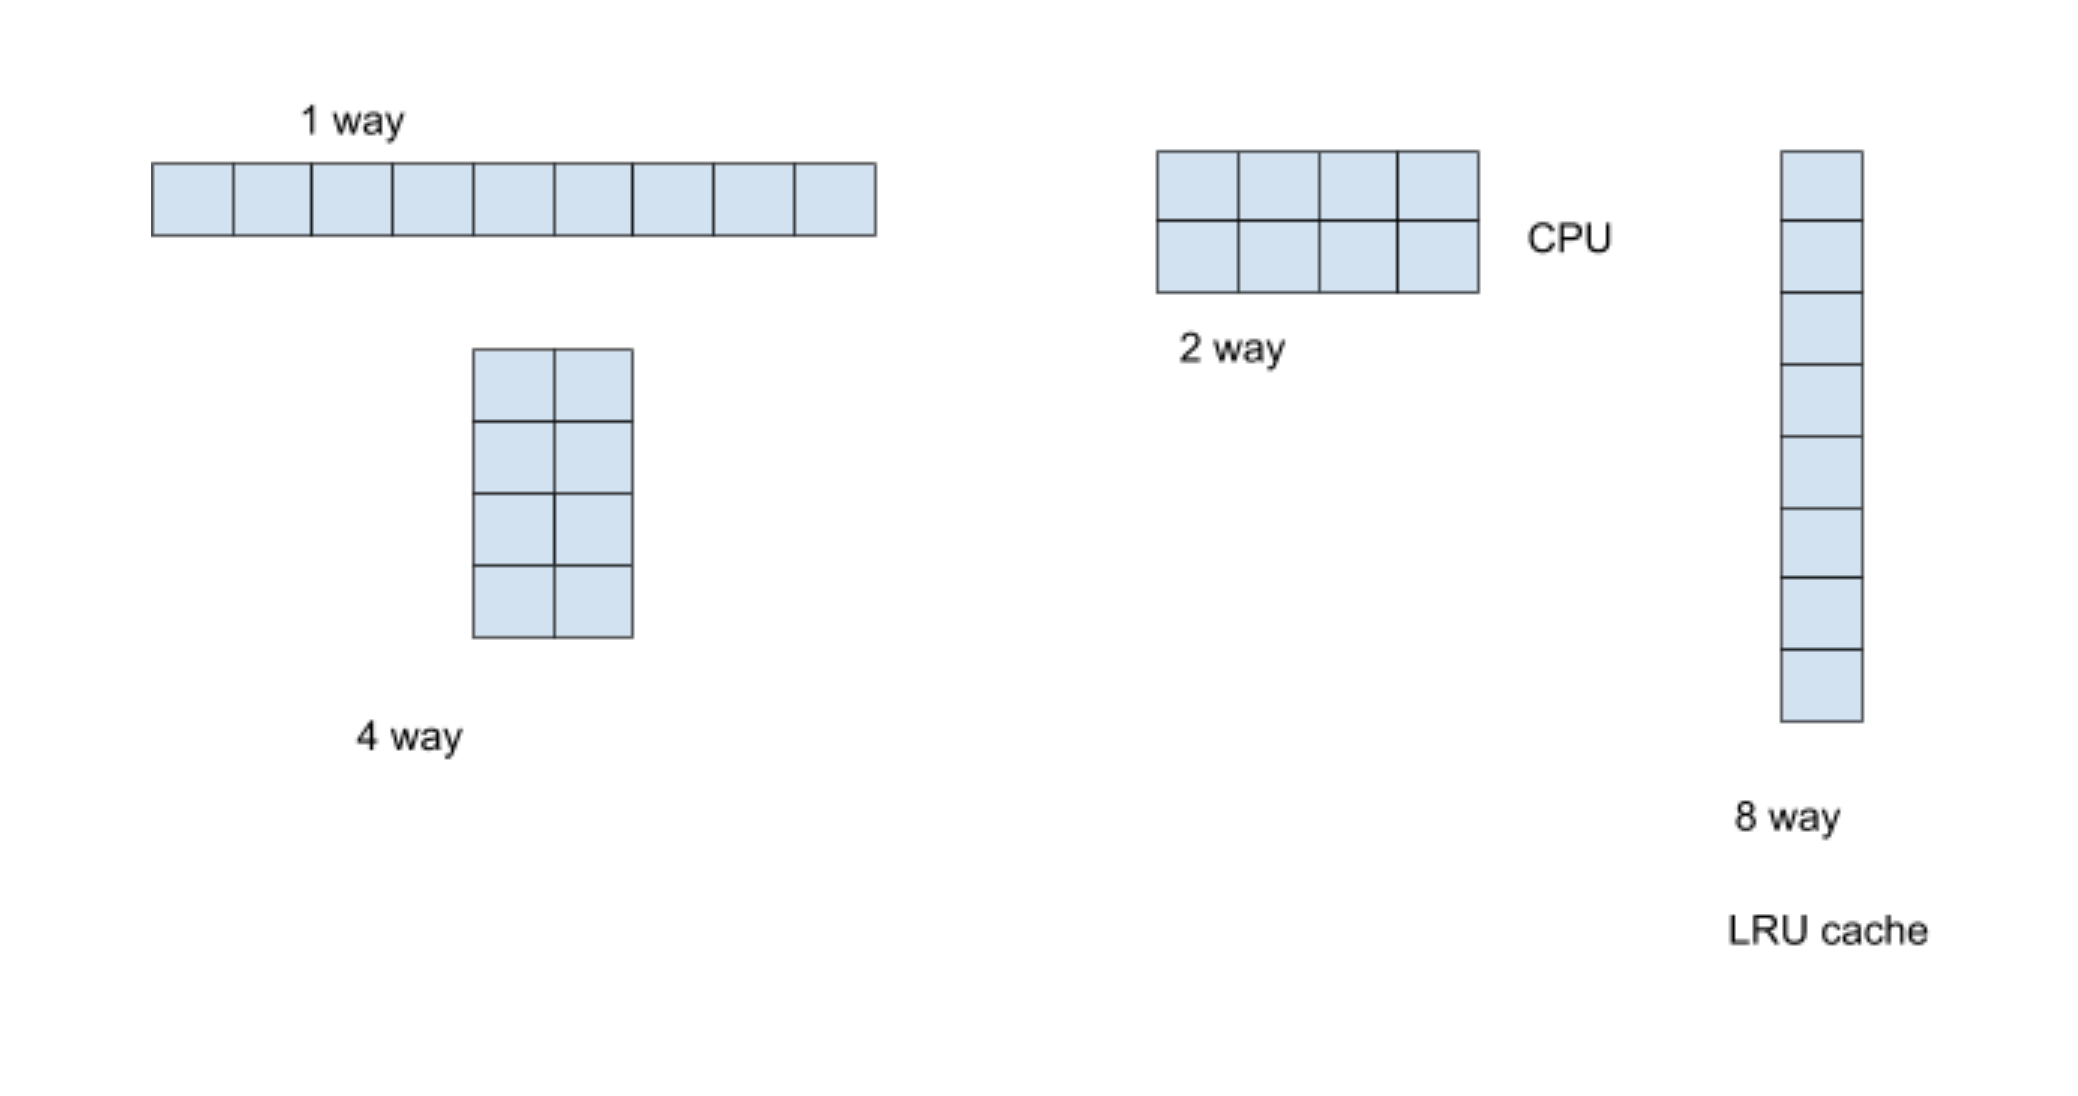
\includegraphics[width=\linewidth]{fig7.png}
  \caption{cache packing}
  \label{fig:fig7}
\end{figure}
These are many degrees of packing that goes on when you divide up all caches. 
\newline
Direct Mapped (1-way)\newline
2-way\newline
4-way\newline
8-way\newline
16-way\newline
Fully associative (infinity way)\newline
Going down the hierarchy the caches lengths are halved and they are made twice as tall. In the case of a hash collision you store the values in the bins. In the 1 way hash if everything hashed to the same bin that would be really bad because it can only hold one value. In the 4 way case there are 4 spots for collisions. Within each x-way bin you perform LRU.

\section{Translation Lookaside Buffer (TLB)}
This is a fully associative cache because we do not want to have misses in this cache. Fully associative means that data can be stored in any unused space in the cache instead of forcing data to be stored into specific spots in the cache and there are no conflicts. The TLB is a cache of mappings from virtual to physical addresses. 
\newline
When memory is accessed on a processor,  processes are never actually accessing memory by its real address they are instead accessing it by its virtual address. 


\section{Process Isolation}
\begin{figure}[h!]
  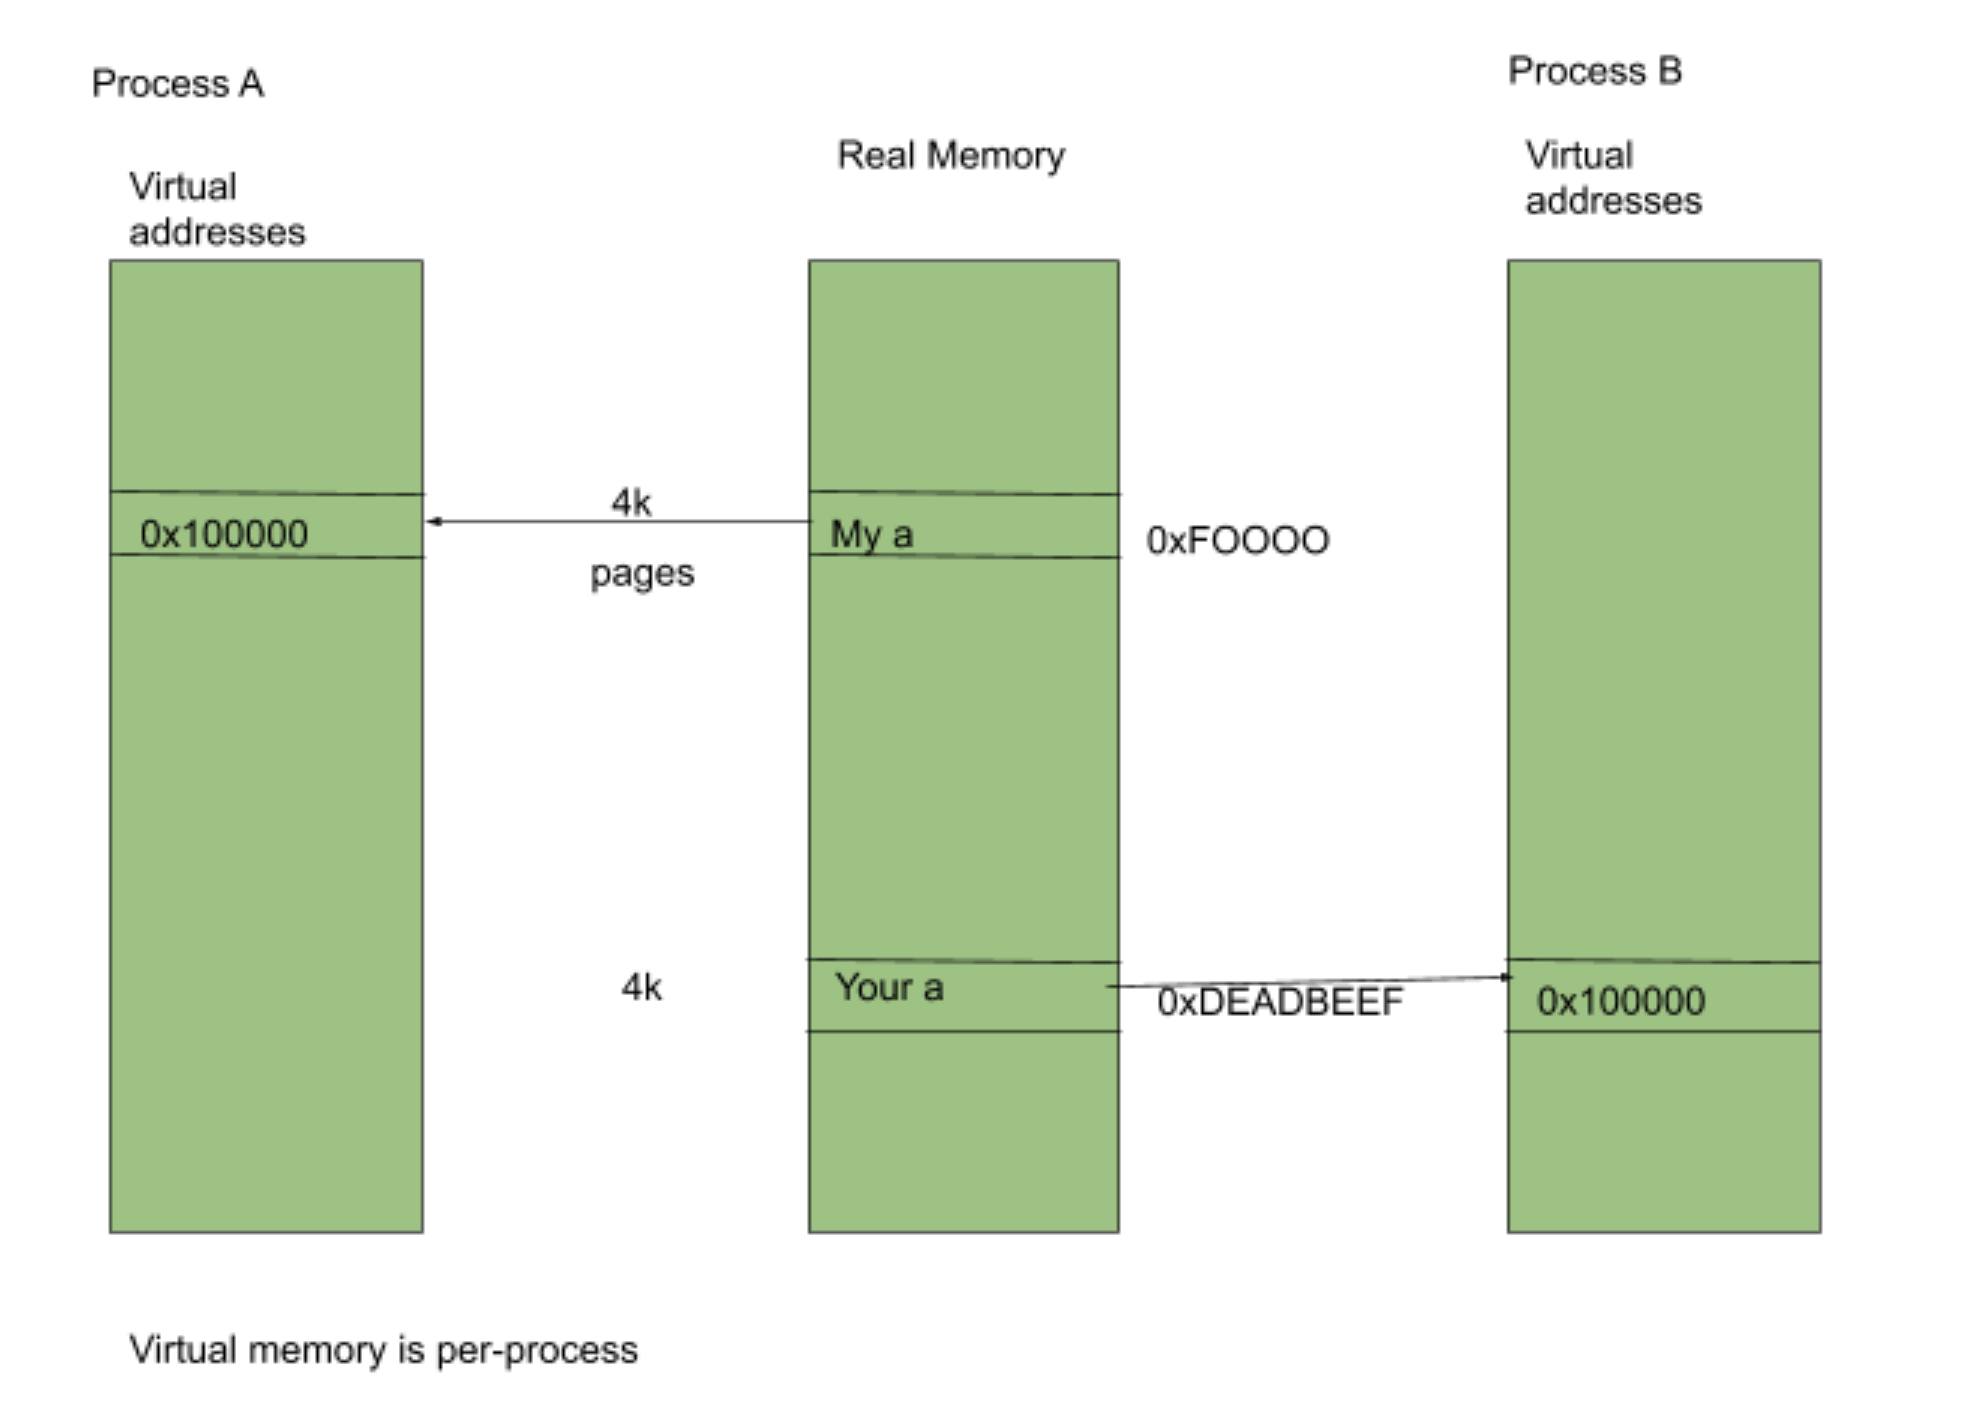
\includegraphics[width=\linewidth]{fig8.png}
  \caption{process isolation}
  \label{fig:fig8}
\end{figure}
Every process has their own view of the world and can never see the content of other processes running on the machine. Pieces of memory from different processes can have the same address because processes use virtual address which are just pretend addresses. 
\newline
\textbf{pages:} real memory holds processes in different chunks of memory referred to as pages and they are a range of memory which have their own unique addresses and are stored in multiples of 4k.   
\newline
Processes create a one per process virtual map referred to as virtual memory which is a mapping of locations in real physical memory to the virtualized memory of the process.  
\newline
\textbf{Page Table:} data structure that is stored in a TLB which contains virtual address to real physical memory address pairs. The structure of this table is defined by the hardware.
\newline
\textbf{Multi-level TLBs:} When data does not fit in the TLB the process has to go to main memory to get the data and that was very slow. TLBs have 1 cycle access time which is very fast and desirable. There are TLBs with multiple levels starting from a smaller TLB ranging down to larger TLBs so we can store more data and avoid going out to main memory. 


\section{Process Switching}
The content of the TLB is also per-process. If a virtual address appears in the TLB it means the process has access to it (it works like a key) this is referred to as capability. Very important when we change from one process to another process they do not get access to each others addresses.
\newline
\textbf{Invalidate TLB entries}: Go through the TLB and invalidate all addresses from old process and load in valid addresses from new process. 
\newline
\textbf{TLB Flush}: When there is a process switch and the TLB needs to get cleared it discards all entries from the previous process and loads the new process.
\newline
Invalidation is good in the case of 2 processes sharing TLB back and fourth and one of them needs access to lots of memory and the other needs access to just a few things. This is better than performing a TLB Flush because you don't have to re-load all memory for the expensive process just go through and re-validate those entries in the TLB saves time going back to main memory.  

\section{Scheduling}
\begin{figure}[h!]
  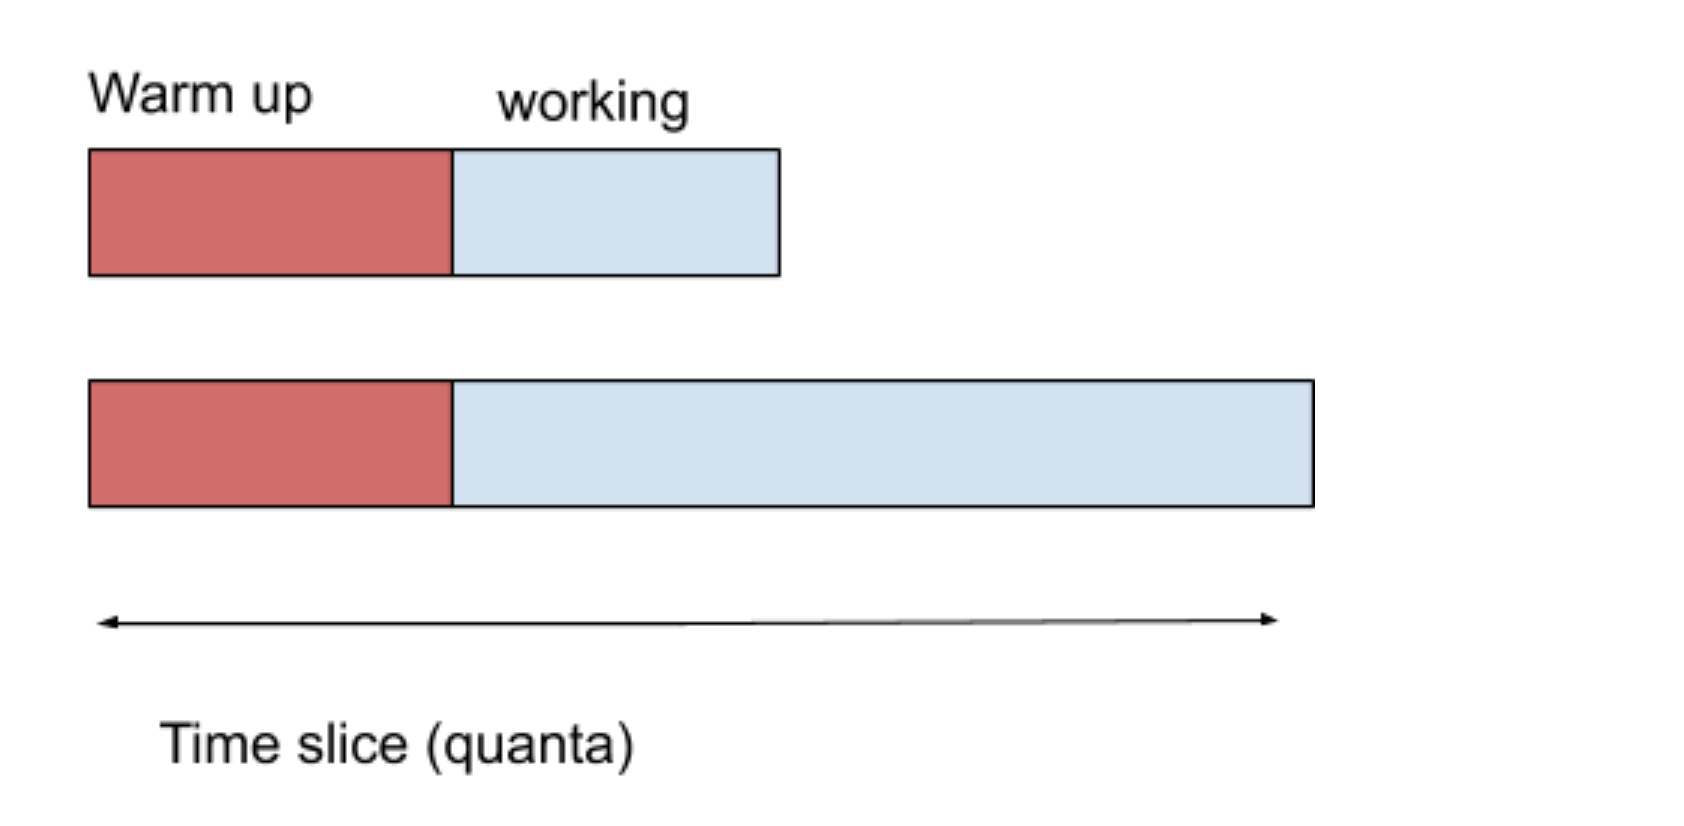
\includegraphics[width=\linewidth]{fig9.png}
  \caption{scheduling}
  \label{fig:fig9}
\end{figure}
\textbf{Time Slicing:} The CPU constantly is switching between processes allowing each process to run for a certain amount of time and that is how scheduling works.
\newline
This amount of time is hard to chose because we want to minimize the slice of time per process but at the same time each process needs warm up time to fill its caches and TLBs but also to needs to have time to perform some tasks. With warm up time in mind, if this slice of time is too narrow the processes will warm up and be short on time to perform tasks. If this time slice is too long processes get too much time on the CPU and other processes get stuck waiting. There has to be a perfect balance so we wish to amortize the warm up across the time quanta. Multi cores fix this issue because the machine could be warming up for some processes and running other processes at the same time. 
\newline
This switching is known a context switch and the cost of warming caches up is referred to as context switch overhead
\newline
Context switch overhead is  high for processes and low for threads. This is because in the case of threads the TLB only has to to save registers and all the process state stays the same so there is practically no context switching overhead. 
\newline
\textbf{Warming up the cache:} When processes are given their turn on the CPU they need to get a bunch of memory from main memory referred to as a "working set" onto their cache. 
\newline
\textbf{Cold Cache:} The cache for a freshly loaded process is empty and its called cold cache.

\section{Registers:}
There is a fixed number of registers example: A B C D
\newline
There is some number of variables in your program example: x y z a b c q r s
\newline
We do not have a register for every variable (registers $<$ variables) so we must figure out which copy of variables get stored in which registers and when to switch them out for other variables.
\newline\newline
\textbf{Register allocation:} maximise the number of time variables are held in registers. When things do not fit in registers the contents of that register would have to be written out to main memory in order to allow other variables to use that register. This is kind of like scheduling.
\newline
\textbf{Spill:} copy contents of register to main memory (eviction)
\newline
If the program is straight line code register allocation is predictable and this is reduced down to a graph coloring problem which is NP complete. For small problems NP complete is fine but for high numbers NP complete is not good.

Linear scan: scan through the registers once and assign registers. If there is a register available use it and if there isn't one available evict the one that was used least recently and use its spot(kind of like LRU). 
\end{document}
